\chapter{Đóng góp và đề xuất}
Đề xuất trong \cite{lu2014construction} sử dụng giải thuật JPSO, là một biến thể của PSO trong miền không gian rời rạc, để giải quyết bài toán đã nêu trong chương trước. Đề xuất sử dụng mã hóa hai lớp, tạo ra hai nhược điểm chính. Thứ nhất là sự phức tạp. Lớp thứ nhất là một dãy nhị phân có độ dài tương ứng với số lượng nút trung gian trong mạng cảm biến, với giá trị 0 là không tồn tại trong lời giải và 1 là ngược lại. Lớp thứ hai là lời giải thực tế được mã hóa thành một cây khung. Sự phức tạp thể hiện ở việc trong quá trình thực hiện giải thuật, cần có một bước đặt biệt để đảm bảo tính thống nhất giữa hai lớp. Việc xây dựng lớp thứ nhất từ lớp thứ hai như một phương án khắc phục đã tạo nên nhược điểm thứ hai của đề xuất là tốc độ thực hiện bị giảm đi khi mất một giai đoạn chuyển đổi.


Hai nhược điểm nêu trên được khắc phục với giải pháp đề xuất trong đồ án, được xây dựng từ giải thuật di truyền. Giải thuật di truyền tổng quát có trình tự như sau:

\begin{algorithm}[bth]
\caption{Giải thuật di truyền}\label{euclid}
\begin{algorithmic}[1]
\Procedure{Giải thuật di truyền}{}
	\State \textbf{Đầu vào: }Đồ thị không hoàn chỉnh vô hướng G=(V,E) \\
	Nút gốc $v_0 \in V$
		
	\State \textbf{Đầu ra: } Cây Steiner T của G 
	
	\State Sinh n cá thể của quần thể $P_0$
	\For{cá thể $id \in P_0$}{
		Thực hiện giải thuật Kruskal trên tập các cạnh đã xáo trộn để tạo thành một cây; \\
		Thực hiện quy trình sửa chữa để thu được cây Steiner; \\
		Tính toán hàm phạt của $id$;
	}
	\EndFor
	$t\leftarrow 0$\\
	\While{điều kiện dừng chưa thỏa mãn}{
		$Q_t \leftarrow$ Thực hiện lai ghép và đột biến trên $P_t$; \\
		$R_t \leftarrow Q_t \cup P_t$; \\
		$P_{t+1} \leftarrow$ Chọn n cá thể tốt nhất từ $R_t$; \\
		$t \leftarrow t+1$;
	}
	\EndWhile
\EndProcedure
\end{algorithmic}
\end{algorithm}

Các bước tiến hành giải thuật sẽ được nêu cụ thể trong các chương sau.

\section{Biểu diễn cá thể}
Giải thuật sử dụng tập cạnh để biểu diễn một cá thể.

\begin{figure}
	\centering
	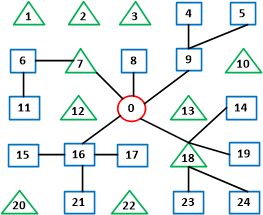
\includegraphics[scale=1.0]{figures/graph}
	\caption{Mã hóa một cá thể}\label{fig:encode}
\end{figure}

Hình \ref{fig:encode} mô tả mã hóa của một cá thể. Tập cạnh biểu diễn là: \{(0,7), (0,8), (0,9), (0,16), (7,6), (6,11), (9,4), (9,5), (16,15), (16, 17), (16,21), (18,14), (18,19), (18,23), (18,24)\}.


Việc mã hóa này đảm bảo một số tính chất quan trọng. Thứ nhất là tính bao quát, tất cả các lời giải khả dĩ đều có thể mã hóa được. Thứ hai là tính duy nhất, mỗi mã hóa chỉ có thể giải mã thành một lời giải duy nhất và ngược lại. Hơn thế, mã hóa sử dụng tập cạnh hỗ trợ thực hiện các nhiệm vụ khác như lai ghép, đột biến mà không cần chuyển đổi, do đó rút ngắn thời gian tính toán so với giải thuật đề xuất trong \cite{lu2014construction}.


Để xây dựng một cây từ tập E ban đầu, trước hết ta áp dụng Kruskal, nhưng thay vì với tập các cạnh được sắp xếp theo độ lớn tăng dần, ta sẽ sử dụng tập cạnh được xáo trộn để tăng tính đa dạng của toàn quần thể. Giải thuật Kruskal có thể dừng lại nếu tất cả các nút cảm biến đều đã được duyệt qua, và áp dụng một quy trình cắt tỉa các nốt thừa (các nốt lá không phải nút Steiner) để thu được một lời giải hợp lệ.
